\paragraph{to add}
In addition to coreset sampling, we could also run on the whole feature, 

\section{Performance Measurements and Results}

\subsection{Performance metrics}
There are three common performance metrics, we have our own way to measure:
\begin{itemize}
    \item Execution time: one is run-time, the other is normalized instance hour;
    \item Memory-consumption \& number of machines: peak memory of mapper and reducer, see Table \ref{table:m3}. We use m3.2xlarge and one master, two cores;
    \item Solution quality: our project is quite innovative and there is no existing work. We can only compare our results with differnt parameters by topographical world map\cite{world}.
\end{itemize}
Generally, it would take four hours to run on the whole datasets, which is more than 100 instance hours.

\begin{table}[htbp]
    \centering
    \label{table:m3}
    \begin{tabular}{|l|l|l|l|}
        \hline
        Model & vCPU & Mem (GiB) & SSD Storage (GB) \\
        \hline
        m3.medium & 1 & 3.75 & 1 x 4  \\
        m3.large  & 2 & 7.5 & 1 x 32 \\
        m3.xlarge & 4 & 15 & 2 x 40 \\
        m3.2xlarge& 8 & 30 & 2 x 80 \\
        \hline
    \end{tabular}
    \caption{Instance types}
\end{table}

\subsection{Result of recent four decades}
Same as Milestone $3$, we selected the year $1983$, $1993$, $2003$ and $2013$ to show the results. The size of raw compressed dataset is as showing in the Table \ref{table:4year}.

\begin{table}[htbp]
    \centering
    \label{table:4year}
    \begin{tabular}{|l|l|l|l|l|}
        \hline
        Year & 1983 & 1993 & 2003 & 2013 \\
        \hline
        Compressed Size & 155MB & 152MB & 159MB & 166MB \\
        \hline
        Original & 912.4MB & 899.7MB & 960.7MB & 987.2MB \\
        \hline
    \end{tabular}
    \caption{Size of dataset in selected years}
\end{table}

We kept adjusting the parameters until we found the result is resonable. The following pictures are snapshots from $150$ clusters, $500$ iterations. From the pictures we can see that there do exist some pattern in the same region in different years. But generally, the shape of clusters would note be the same.

\begin{figure}[htbp]
    \centering
    \begin{tabular}{c}
        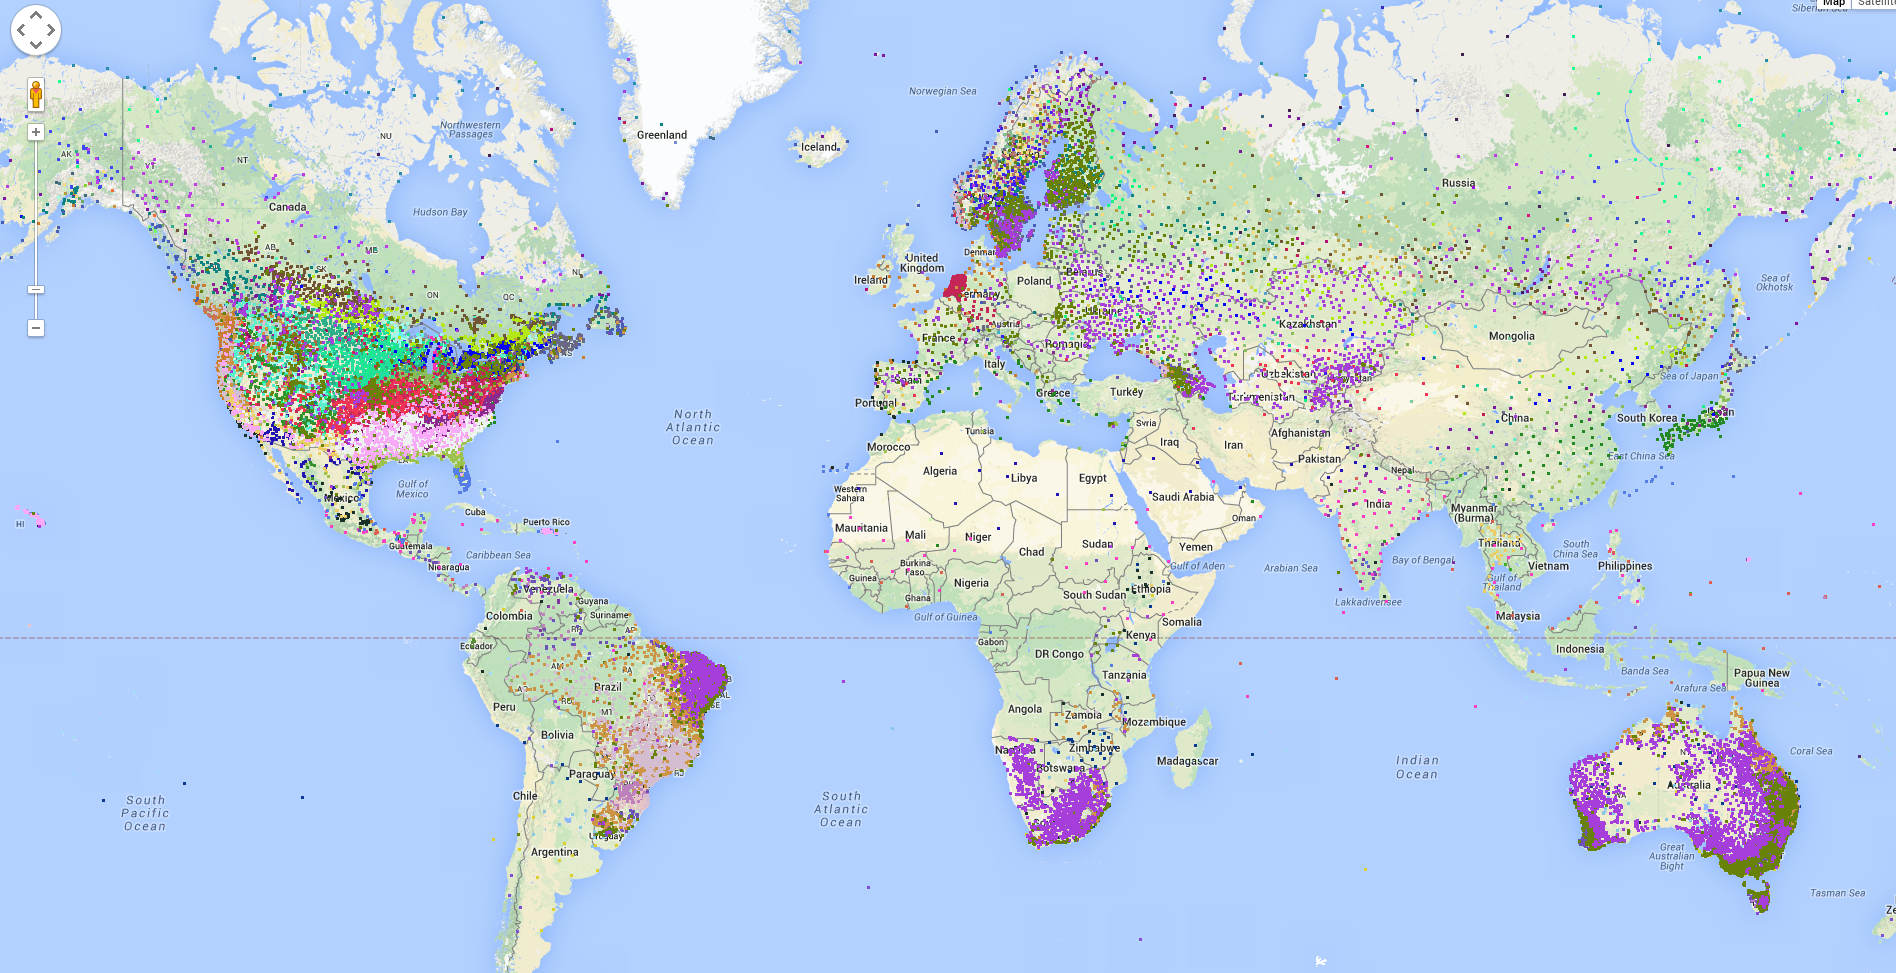
\includegraphics[width =\linewidth]{images/1983.png}\\1983\\
        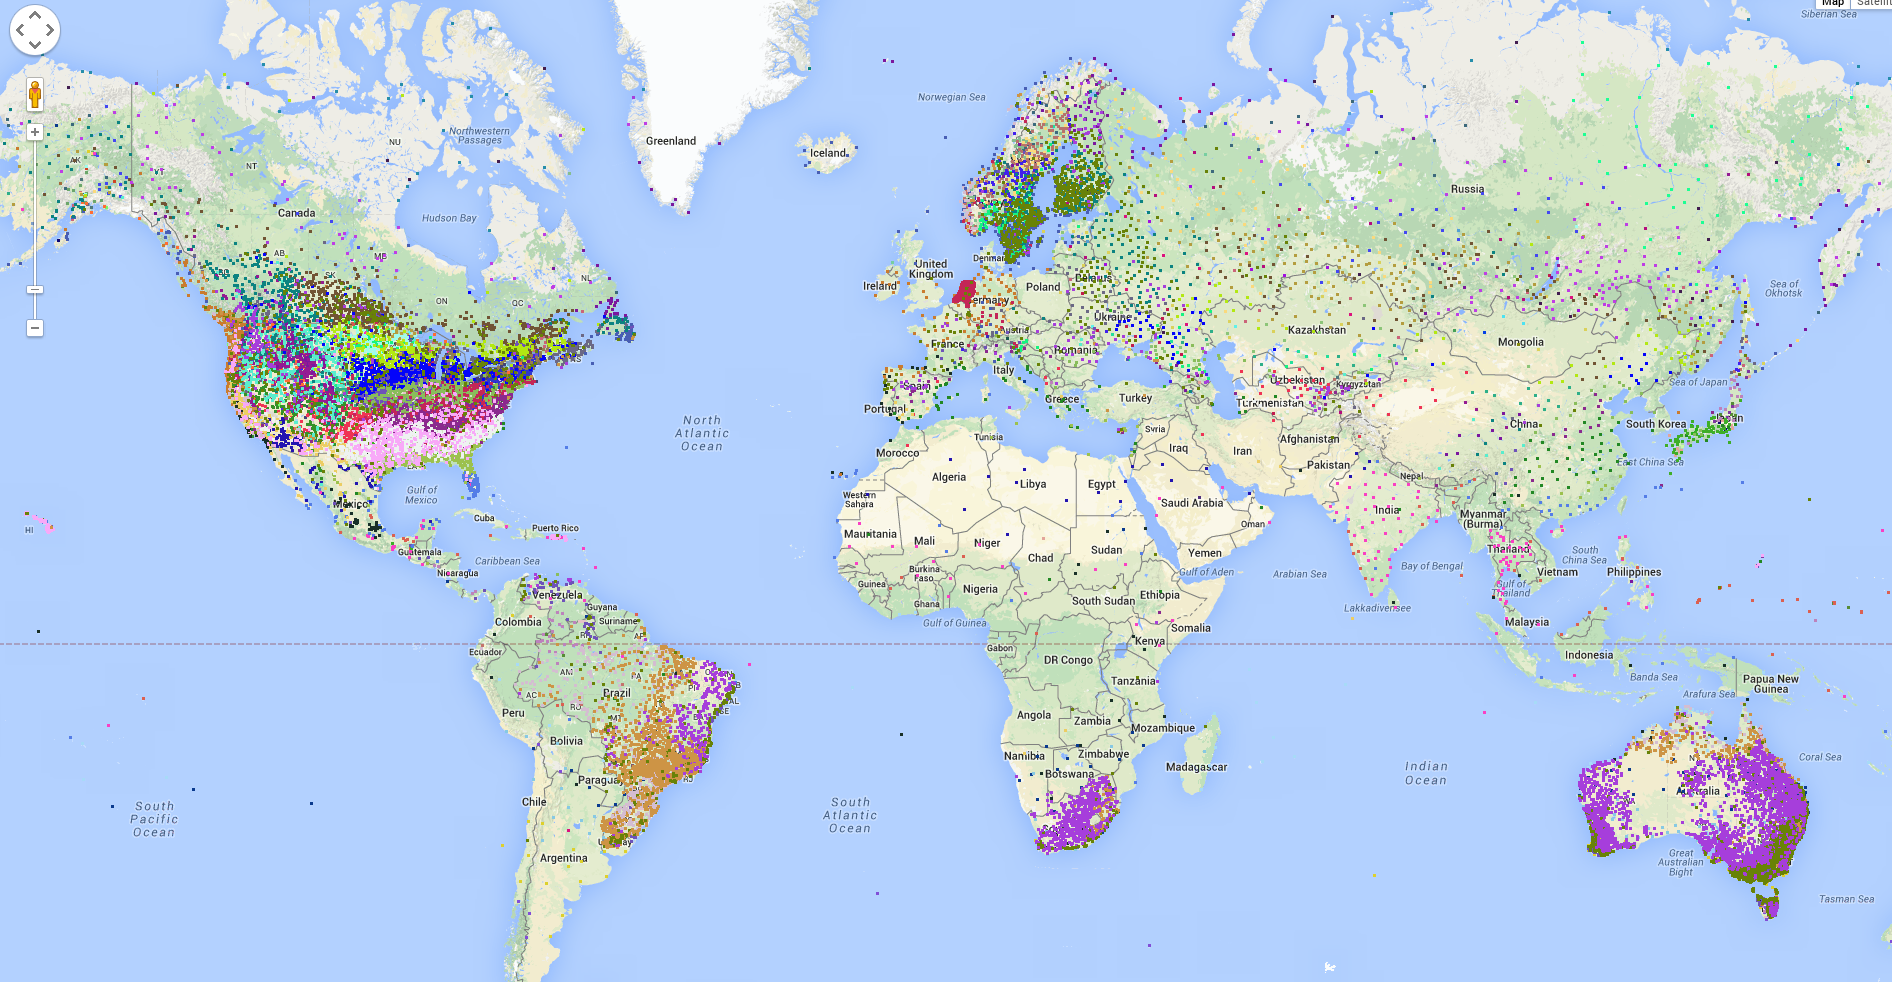
\includegraphics[width =\linewidth]{images/1993.png}\\1993\\
    \end{tabular}
    \caption{Clustering results of 1983 and 1993.}
\end{figure}

\begin{figure}[htbp]
    \begin{tabular}{c}
        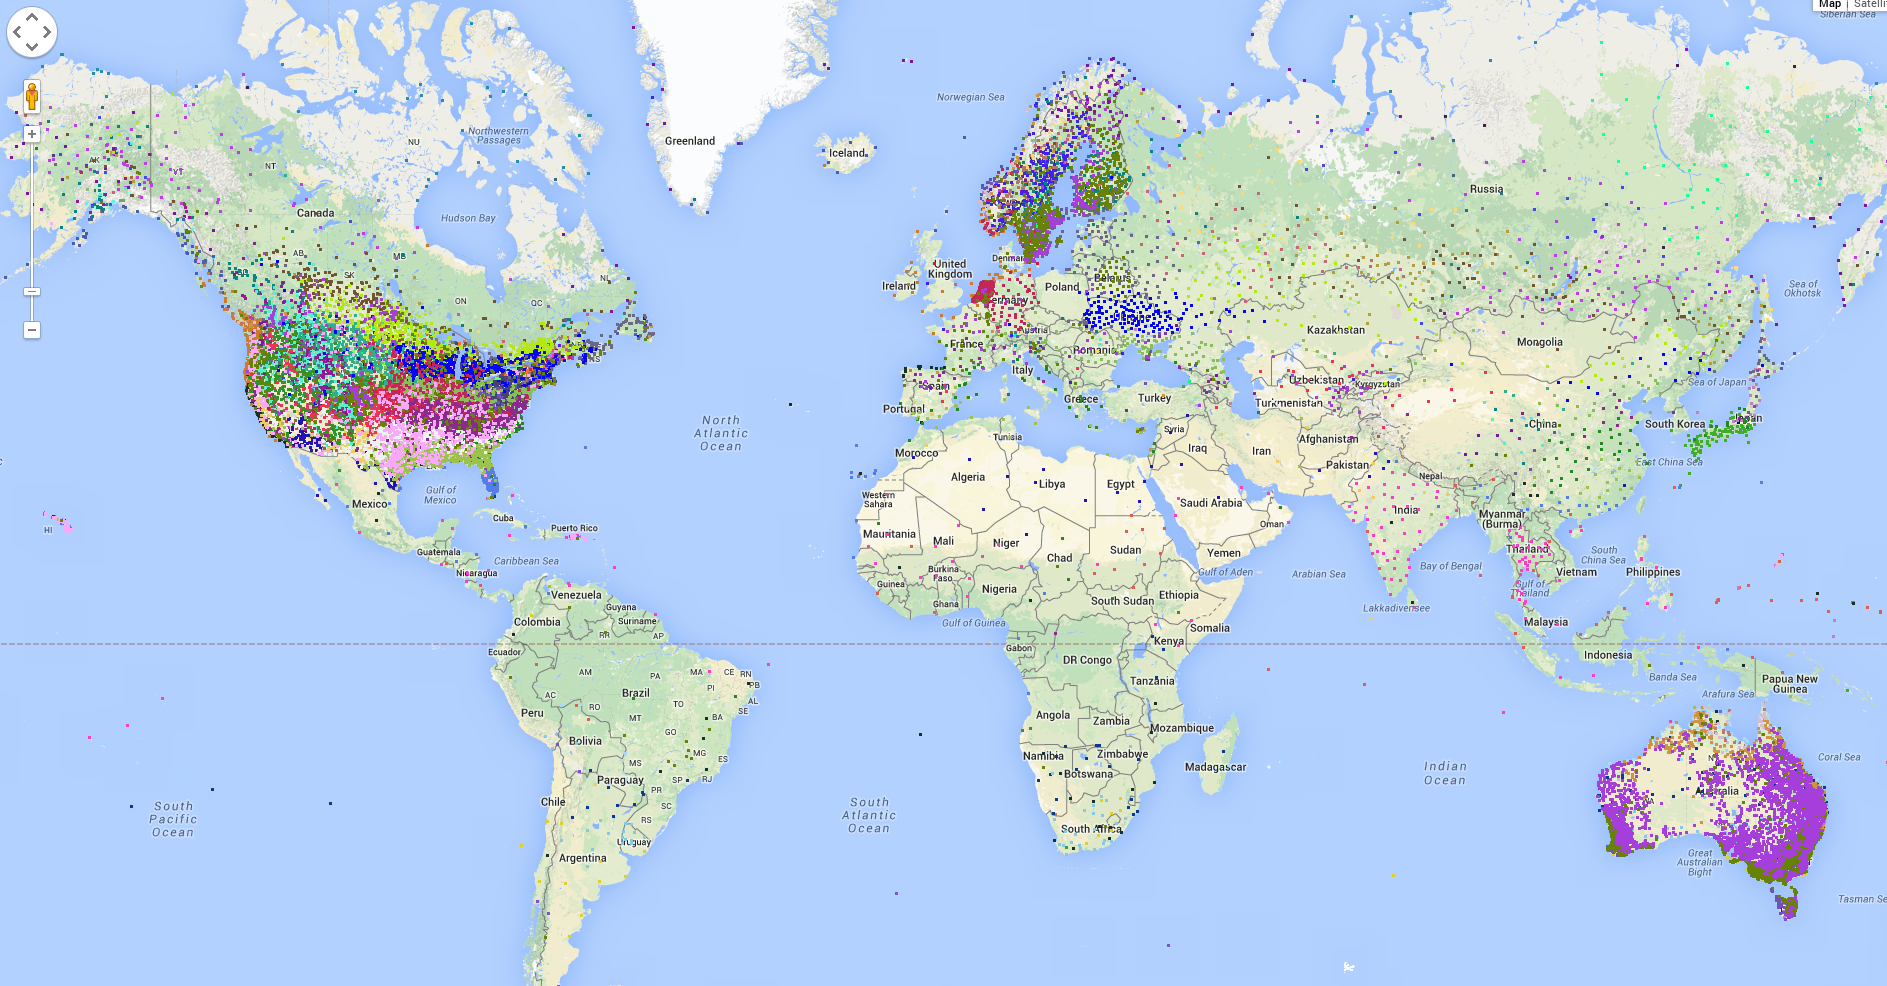
\includegraphics[width =\linewidth]{images/2003.png}\\2003\\
        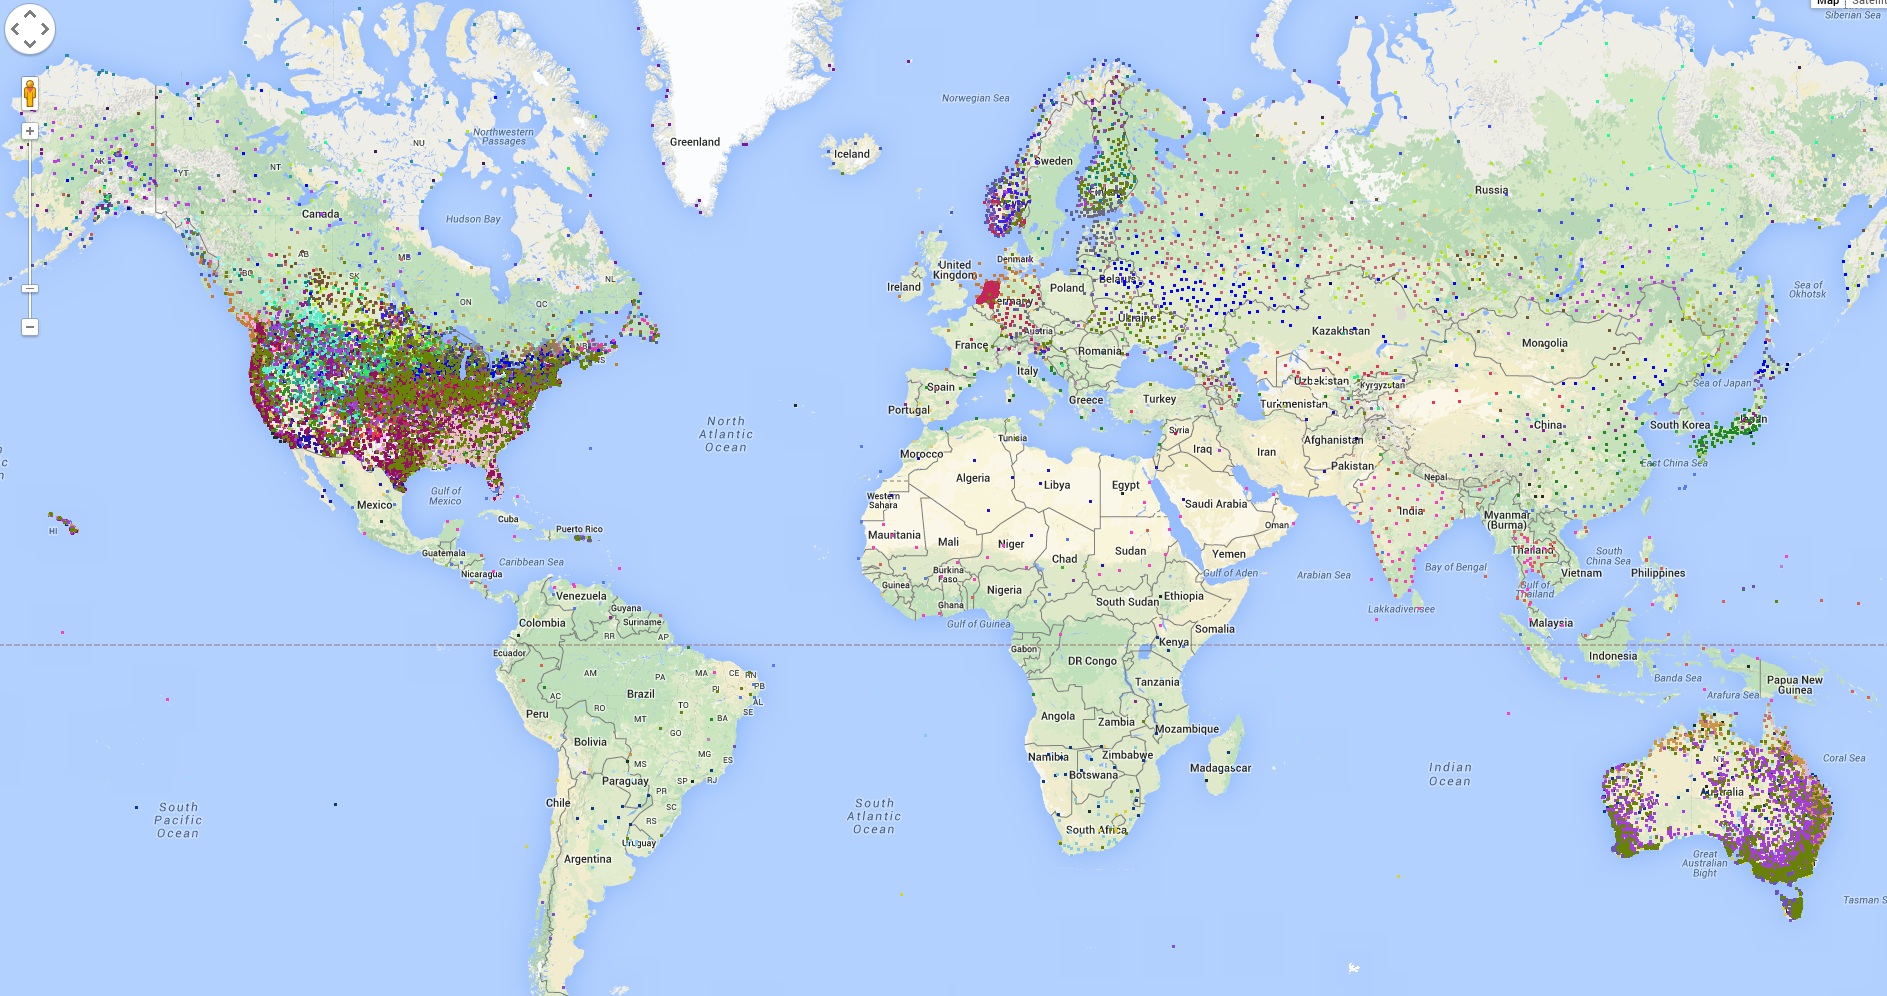
\includegraphics[width =\linewidth]{images/2013.png}\\2013\\
    \end{tabular}
    \caption{Clustering results of 2003 and 2013.}
\end{figure}

Compared with results in milestone $3$, there are two major improvements.
\begin{itemize}
    \item More clusters (which are different colors) are observed;
    \item Less mising points on the map;
\end{itemize}

\subsection{Result of more than a century}

At next step, we adjusted the parameter to less clusters. Because the former years have really small recorded weawther information, it's unnecessary to run many clusters. When we run with $90$ clusters, $500$ iterations to check if there is any similar pattern to the extent of a century. We have chosen the years $1876$, $1896$, $1904$, $1940$, and $2010$ with the size shown in Table \ref{table:5years}. The values are varying from $900K$ to $184M$\footnote{
The results before $1876$ is meaningless since there were not enough data.}.

\begin{table}[htbp]
    \centering
    \label{table:5years}
    \begin{tabular}{|l|l|l|l|l|l|}
        \hline
        Year & 1876 & 1896 & 1904 & 1940 & 2010 \\
        \hline
        Compressed & 900KB & 18MB & 32MB & 73MB & 184MB \\
        \hline
        Original & 5.5MB & 110.2MB & 201.7MB & 441.4MB & 1GB \\
        \hline
    \end{tabular}
    \caption{Size of dataset in selected years}
\end{table}

\begin{figure}[htbp]
    \centering
    \begin{tabular}{c}
        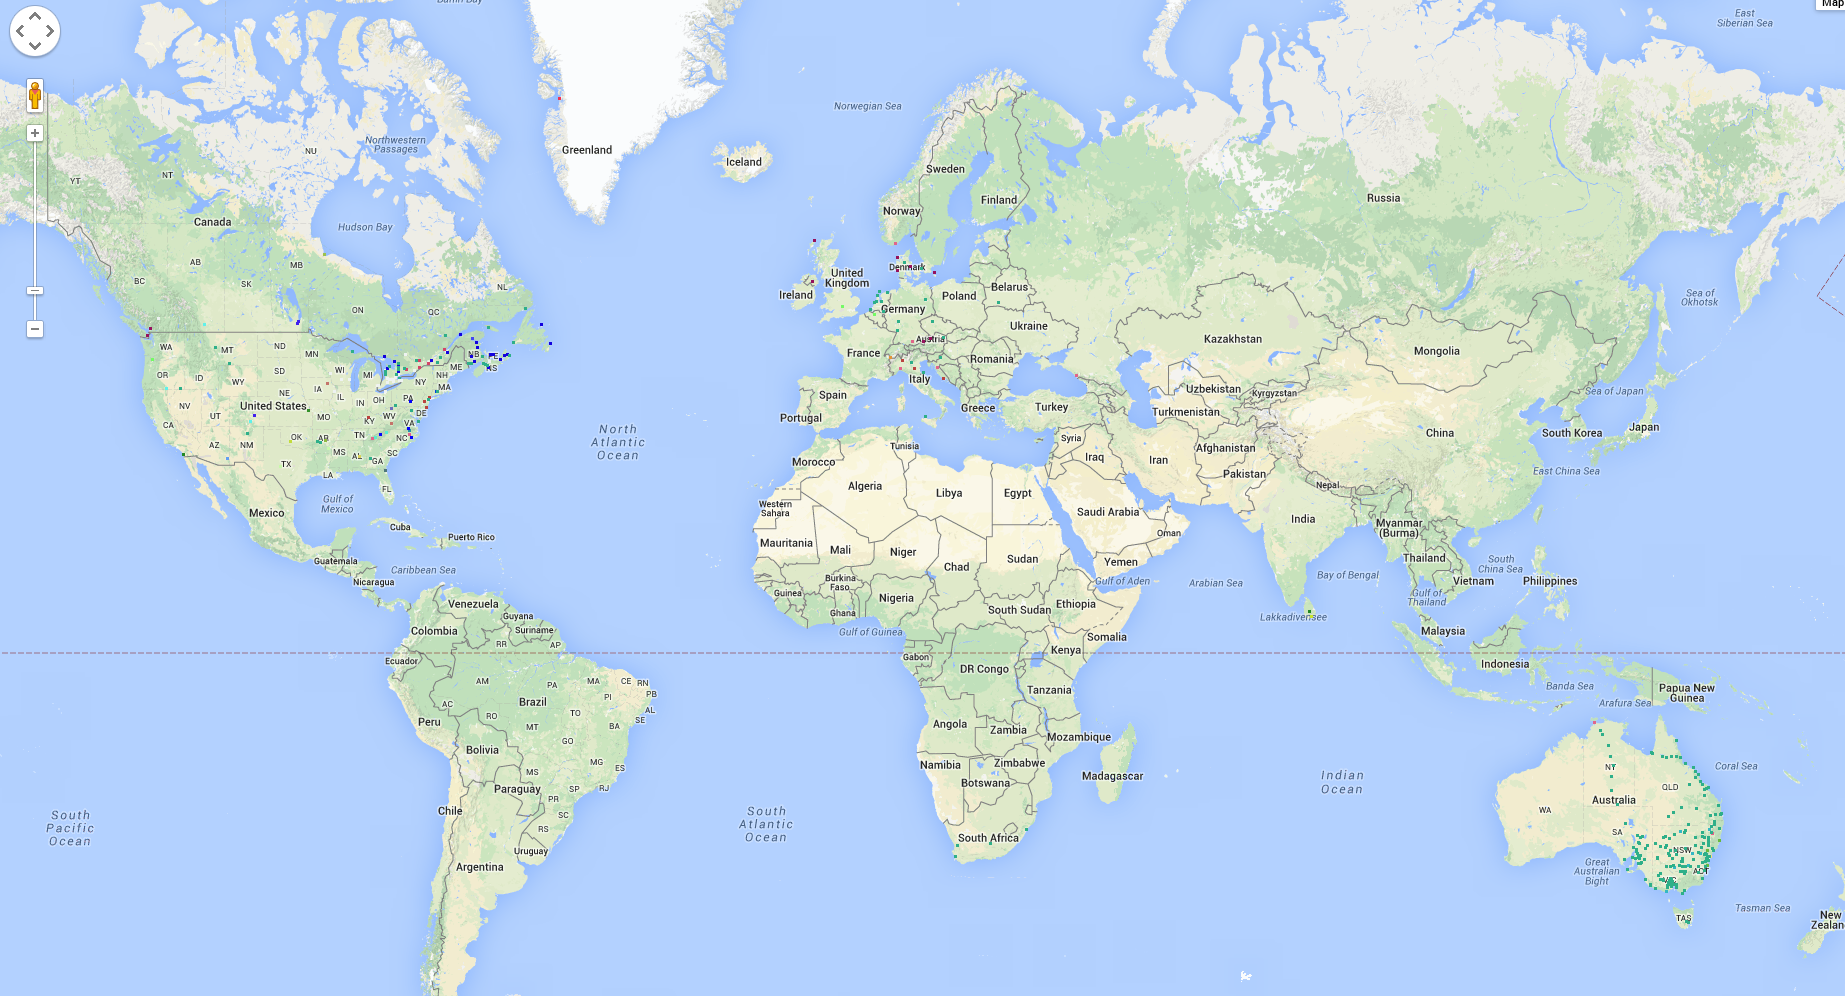
\includegraphics[width =\linewidth]{images/1876.png}\\ 1876\\
        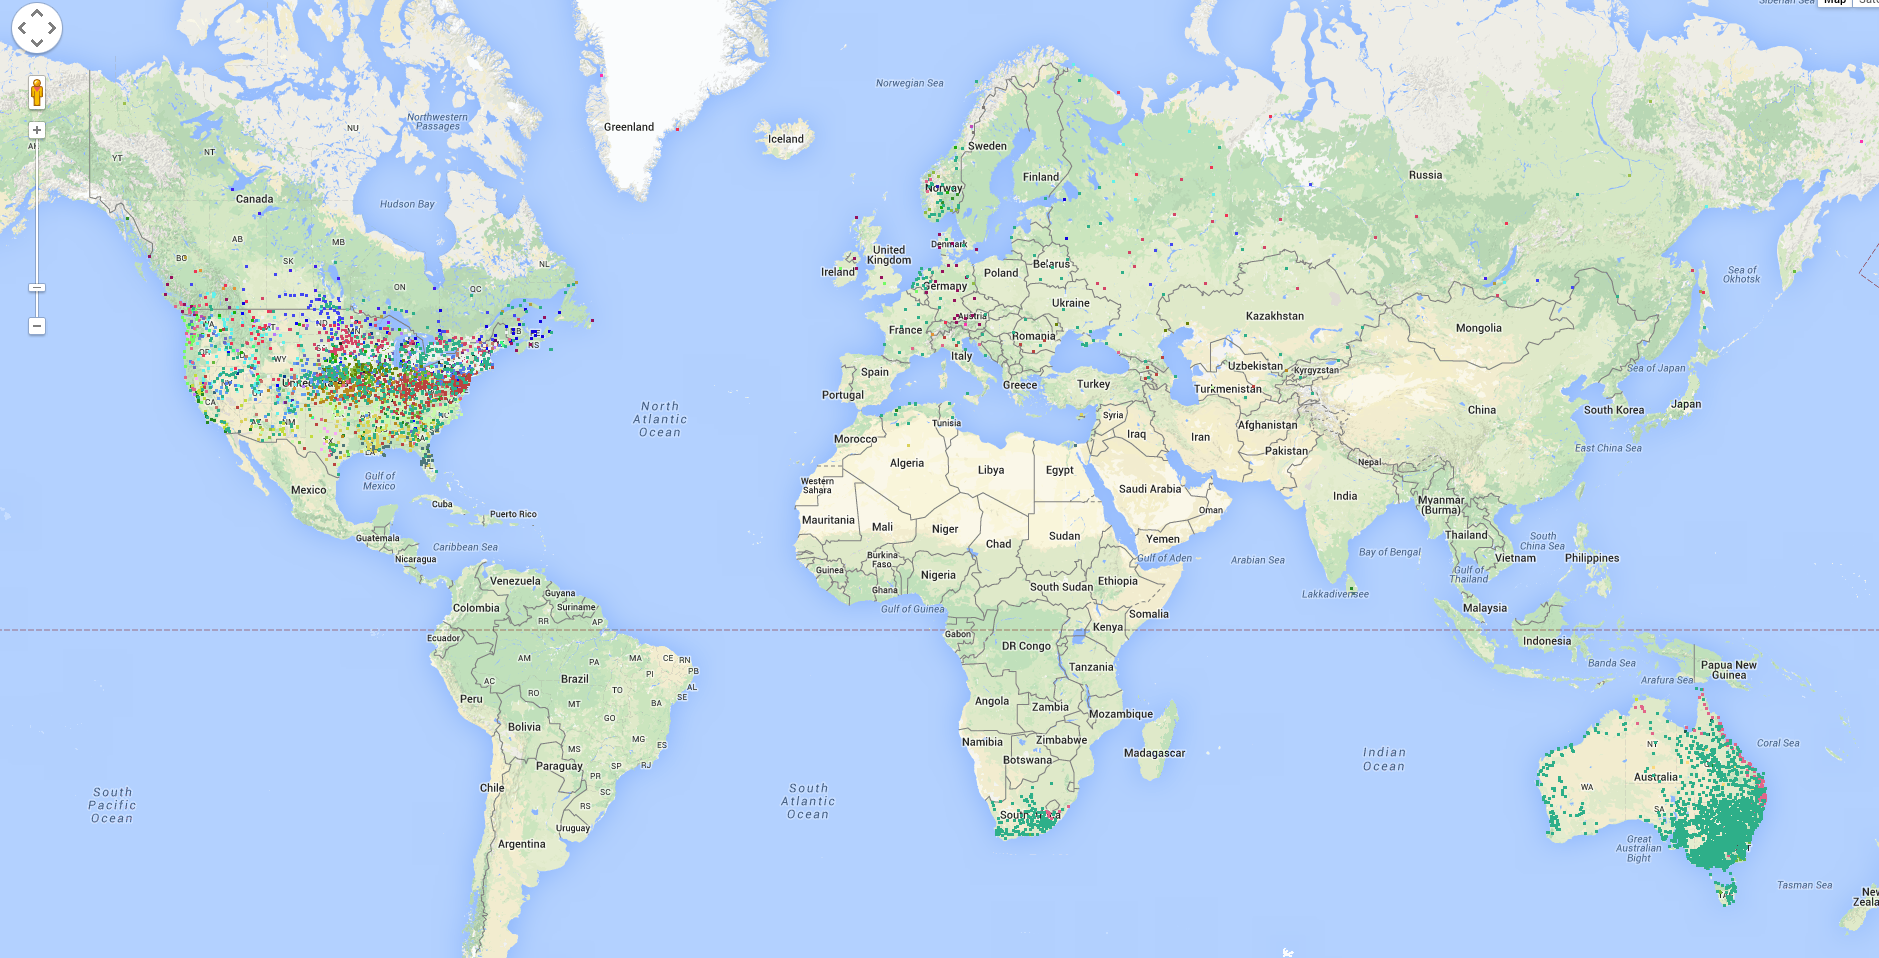
\includegraphics[width =\linewidth]{images/1896.png}\\ 1896\\
   \end{tabular}
    \caption{Clustering results of 1876 and 1896.}
\end{figure}

\begin{figure}[htbp]
    \centering
    \begin{tabular}{c}
        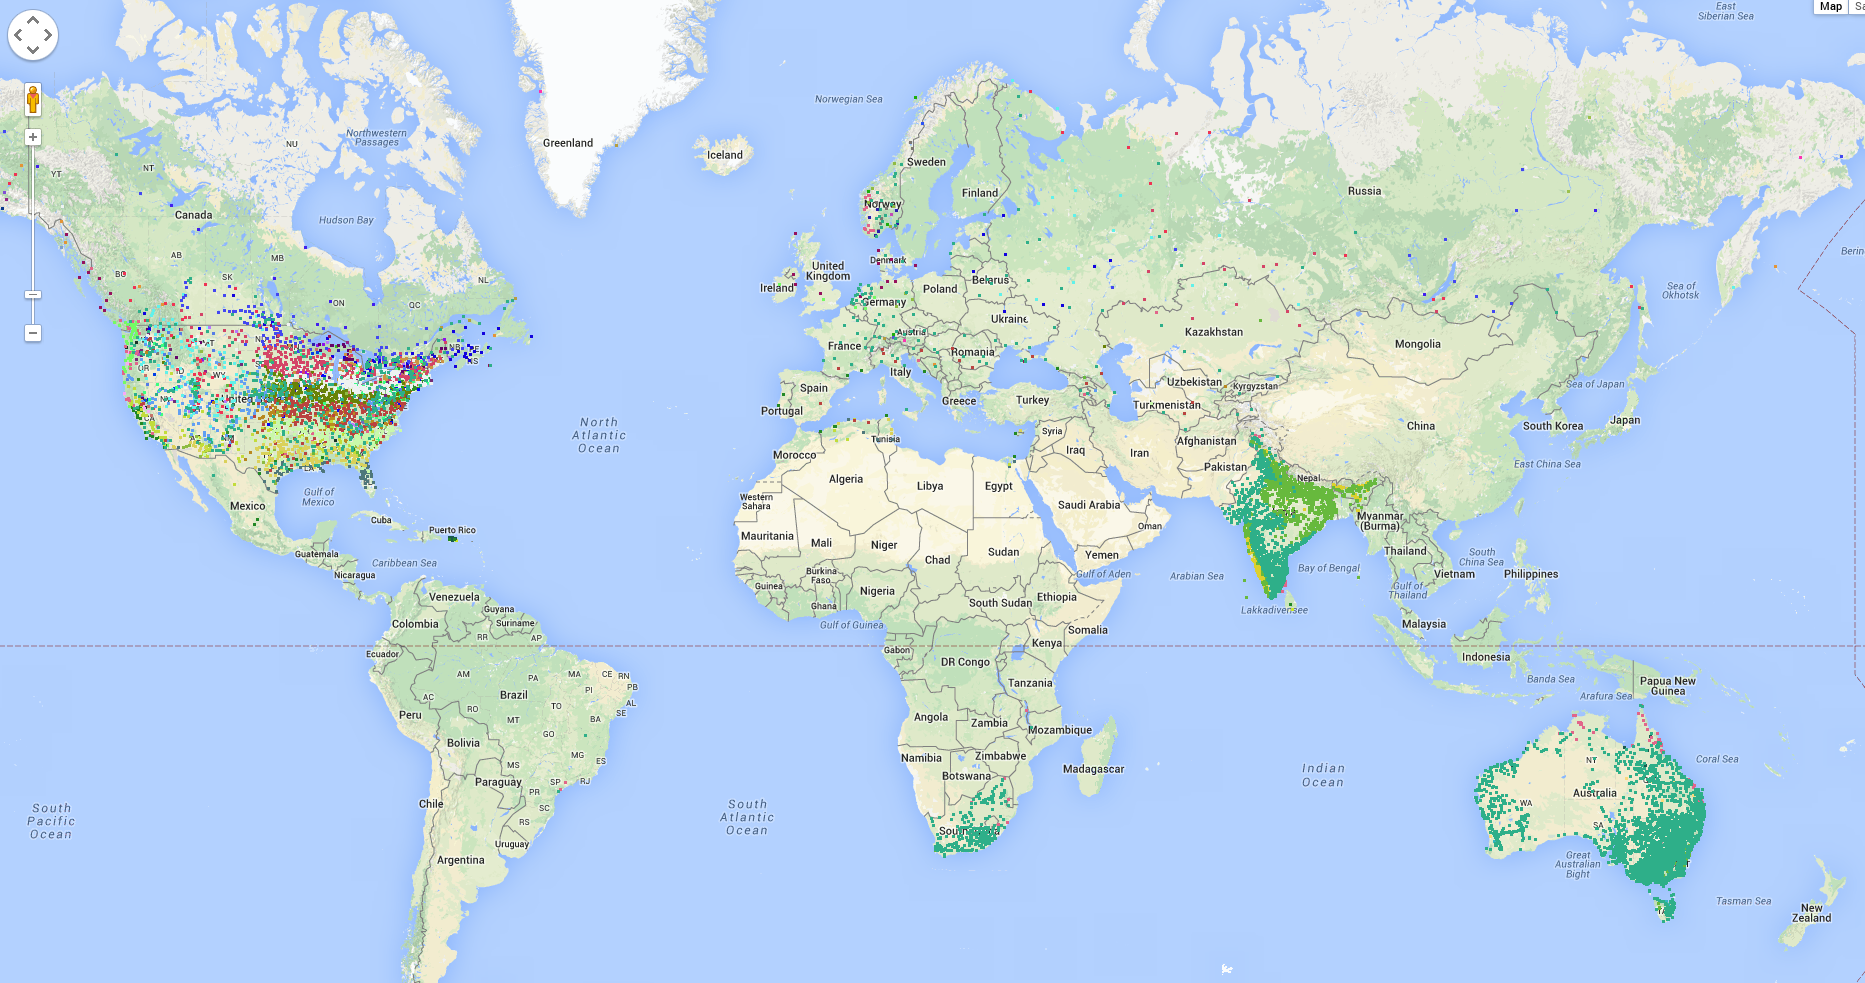
\includegraphics[width =0.8\linewidth]{images/1904.png}\\ 1904\\
        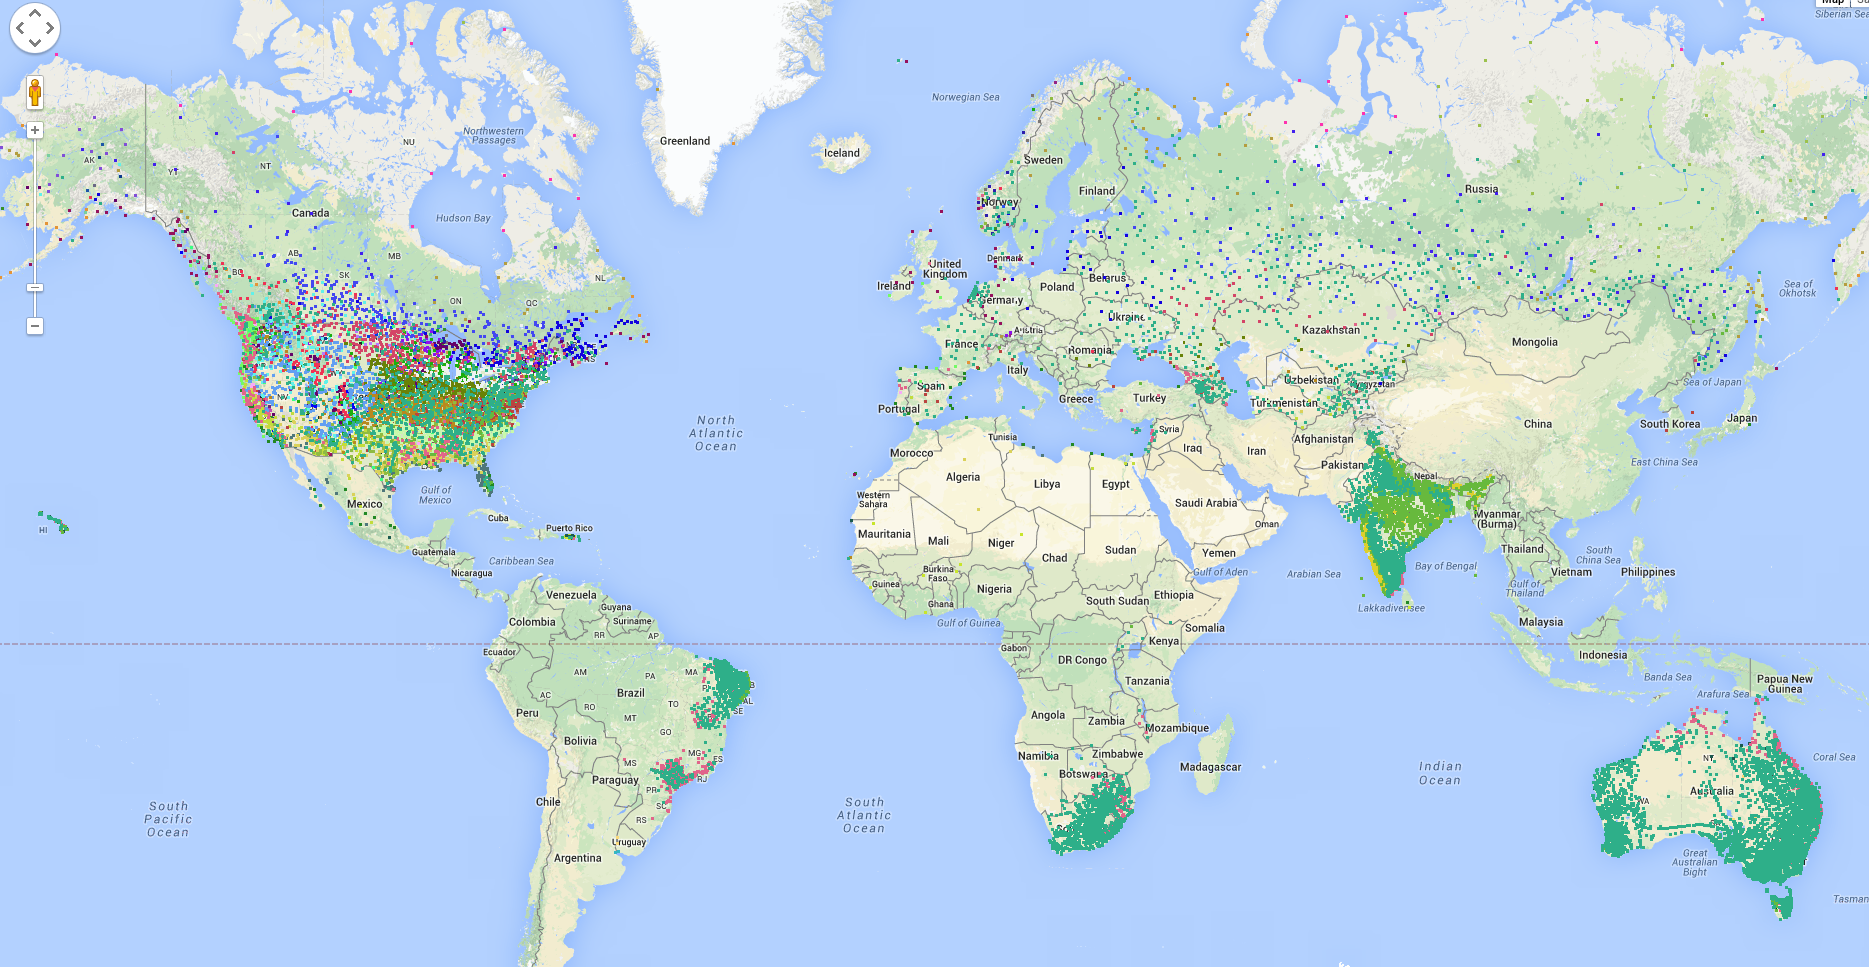
\includegraphics[width =0.8\linewidth]{images/1940.png}\\ 1940\\
        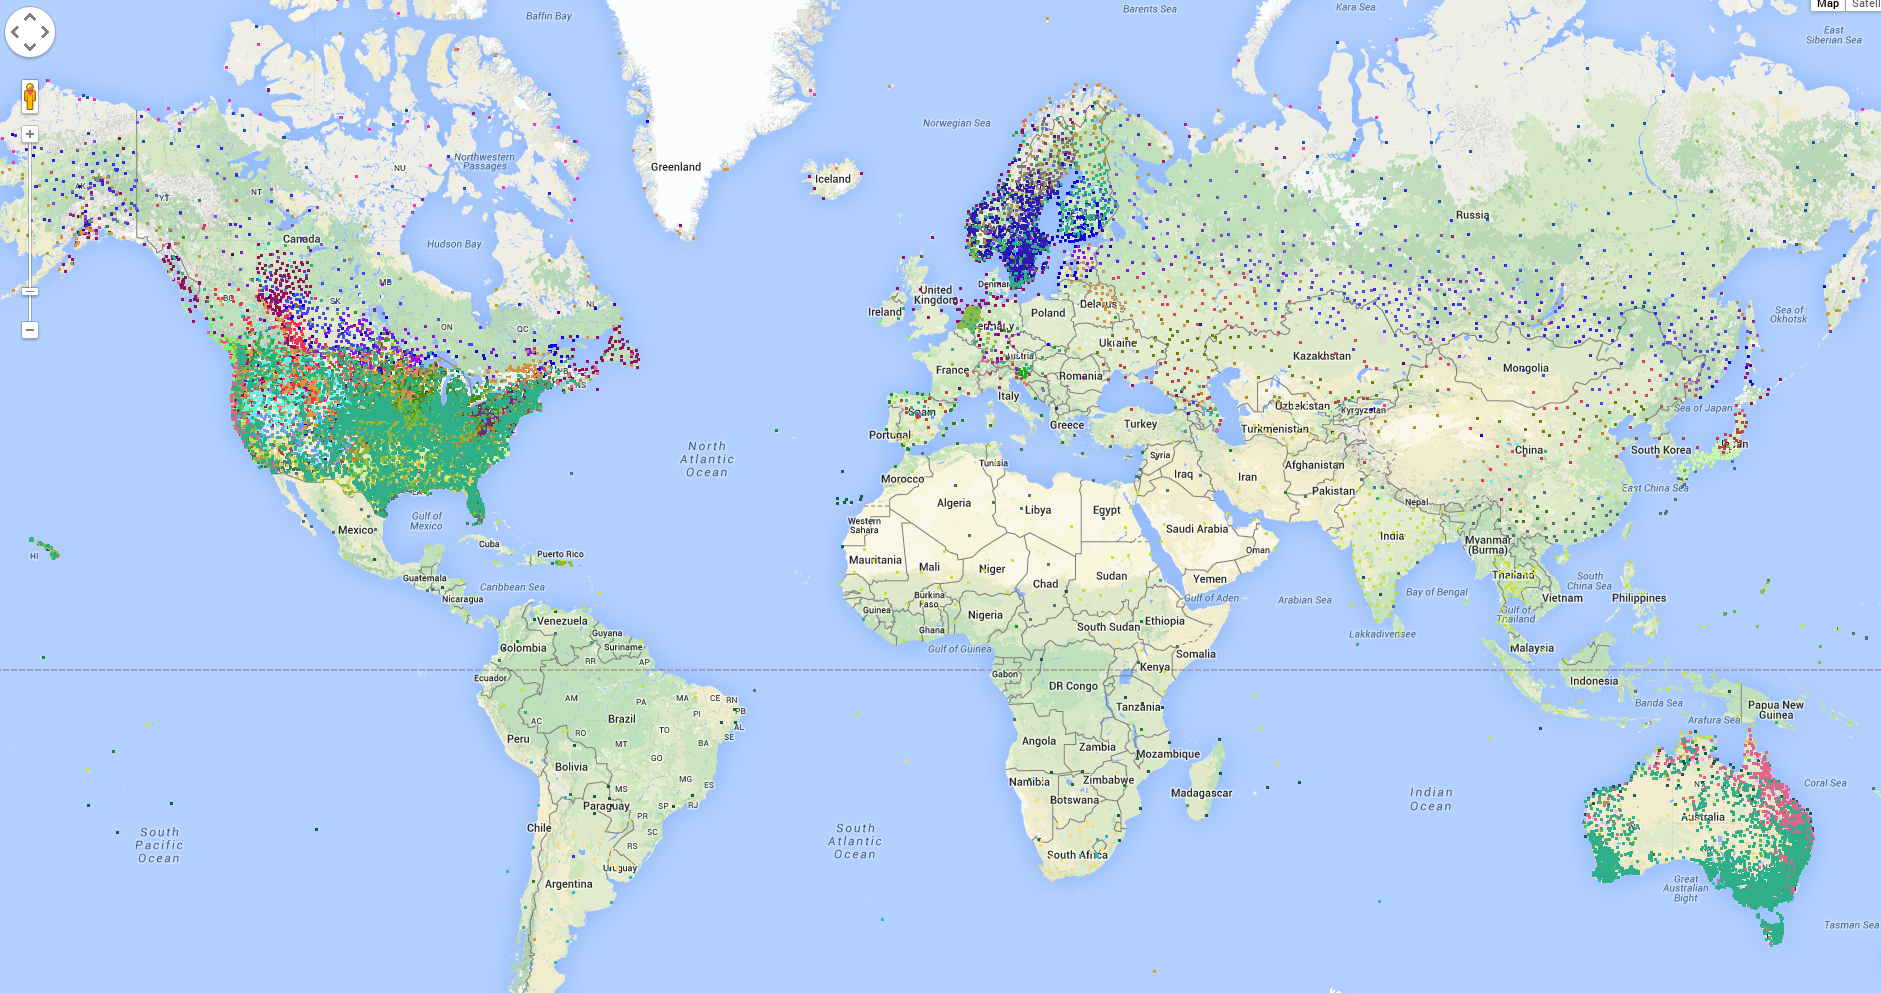
\includegraphics[width =0.8\linewidth]{images/2010.png}\\ 2010\\
    \end{tabular}
    \caption{Clustering results of 1904, 1940 and 2010.}
\end{figure}

Here we observed a similar result as before. 

\subsection{Result of recent $11$ years}

We also extracted the result from $2003$ to $2013$, made a video by Python which is now available on Youtube\cite{youtube}.
